% !TEX root = ../main.tex

\section{Jack Monitor}
\label{sec:jack-monitor}

\scaffold{
  \textbf{Paragraph 1, interface of the monitor.} One \emph{jack monitor} per jack implements \cref{sec:plug-detection,sec:following} as a state machine. It never touches hardware: it hands out one reading at a time (the drive of each of the four contacts, the contact to read, and whether the drive change needs settling) and takes the measured voltage back, together with the time in milliseconds. This lets a scheduler interleave jacks on two ADCs and lets the host tests drive it from a model. It reports a \emph{mode} per jack: empty, identifying, tracking (a potentiometer), switch, rheostat, open (a plug with nothing conducting), or other.
}

\scaffold{
  \textbf{Paragraph 2, states.} Walk through \cref{fig:jack-monitor-states} along the main flow: rails at start-up, empty with a plug check every \qty{50}{\milli\second}, solve (rails re-measured first if older than \qty{30}{\second}), classification, then one of the following states. Then the two ways back: following a potentiometer returns to identification when a track-end check or the wiper range fails, switch, rheostat and open return to empty when the plug check fails. Name the confirm-plug state, which tells an empty jack from an open plug after a solve found no current. Do not describe every edge; the figure does.
}

\begin{figure}[htbp]
  \centering
  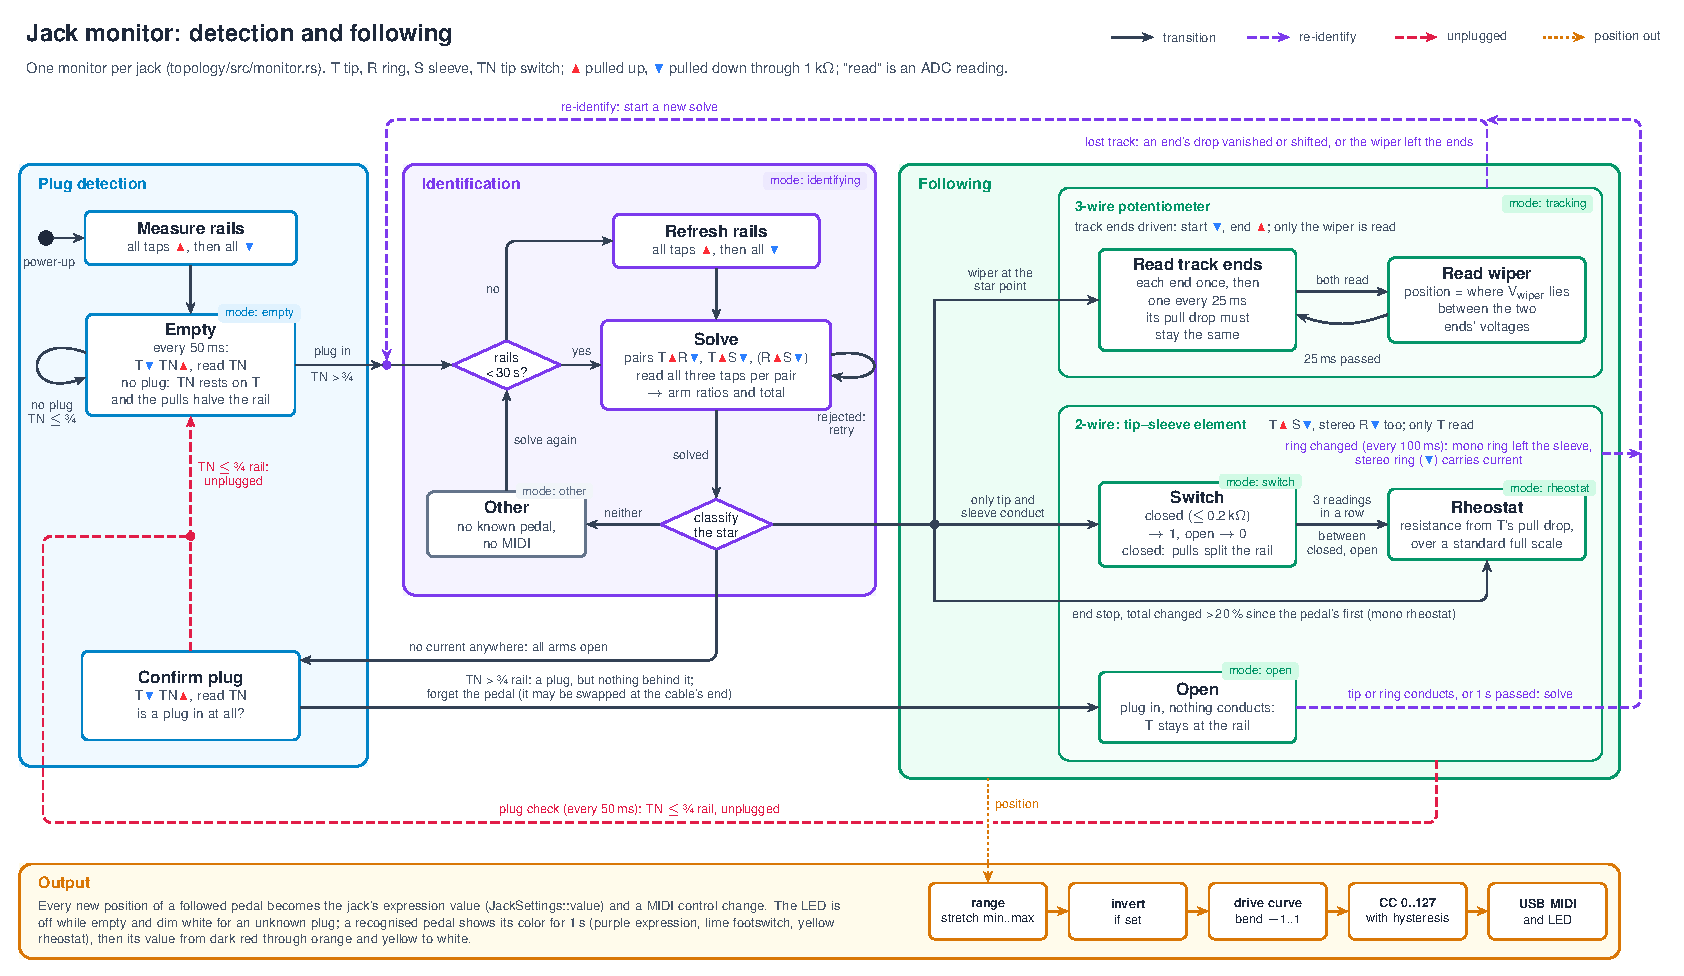
\includegraphics[width=\linewidth]{04-implementation/figures/jack-monitor-states}
  \titledcaption{Jack Monitor State Machine}{\scaffoldinline{Explain the three groups (plug detection, identification, following), the mode tag on each state, the drive symbols (red up, blue down), the two return corridors (re-identify above, unplugged below) and the output strip. Source: \code{docs/diagrams/jack-monitor-states.tex}. Consider a landscape page if the labels are too small at text width.}}
  \label{fig:jack-monitor-states}
\end{figure}

\scaffold{
  \textbf{Paragraph 3, constants.} Present \cref{tab:monitor-config} and point out that every interval and fraction was set or changed by an observation on the board; give two examples from the table with their reason (the \qty{25}{\percent} wiper limit from a pedal with resistance in its wiper lead, \cref{sec:pedal-types}; the \qty{25}{\percent} tolerance of the first track-end reading because solves of a pedal on an end stop were \qty{10}{\percent} off). The remaining reasons are in the appendix (\cref{tab:monitor-config-full}).
}

\begin{table}[htbp]
  \centering
  \titledcaption{Main Constants of the Jack Monitor}{\scaffoldinline{Explain that relative values refer to the total resistance of the network and that $\sigma$ is the noise of the checked quantity. Source: \code{MonitorConfig::new} in \code{topology/src/monitor.rs}.}}
  \label{tab:monitor-config}
  \begin{tabular}{@{}ll@{}}
    \toprule
    \textbf{Constant} & \textbf{Value} \\
    \midrule
    Plug check interval & \qty{50}{\milli\second} \\
    Track-end check interval (potentiometer) & \qty{25}{\milli\second} \\
    Ring check interval (switch, rheostat) & \qty{100}{\milli\second} \\
    Full solve of an open plug & every \qty{1}{\second} \\
    Rail refresh before a solve & after \qty{30}{\second} \\
    Readings averaged per rail & 8 \\
    Plug threshold & \num{0.75} of the rail span \\
    Largest wiper arm & \qty{25}{\percent} \\
    Largest arm at an end stop & \qty{2}{\percent} \\
    End-drop tolerance, first reading / later & \qty{25}{\percent} / \qty{3}{\percent} or $6\sigma$ \\
    Wiper range margin & $6\sigma$ + \qty{0.5}{\percent} of the span \\
    Closed switch & $\leq \qty{0.2}{\kilo\ohm}$ \\
    Readings between open and closed for a rheostat & 3 \\
    Assumed total before the first solve & \qty{100}{\kilo\ohm} \\
    \bottomrule
  \end{tabular}
\end{table}

\scaffold{
  \textbf{Paragraph 4, memory per plug.} What the monitor learns about a plug (that it is a rheostat, the total at its first end stop, the full scale) is forgotten when the plug comes out or turns out open, because a cable left in the jack may get the next pedal at its other end. The wiper of the last potentiometer is kept beyond that, for the next ambiguous end stop in the same jack. Mention the bug that motivated forgetting on an open plug: a stereo cable plugged into the jack first and into a potentiometer pedal afterwards connected tip and sleeve before the ring, was taken for a switch turning into a rheostat, and stayed one, until a ring check for stereo plugs was added.
}
